\documentclass[ignorenonframetext,]{beamer}
\usetheme{Warsaw}
\usefonttheme{structurebold}
\usepackage{amssymb,amsmath}
\usepackage{ifxetex,ifluatex}
\usepackage{fixltx2e} % provides \textsubscript
\usepackage{lmodern}
\ifxetex
  \usepackage{fontspec,xltxtra,xunicode}
  \defaultfontfeatures{Mapping=tex-text,Scale=MatchLowercase}
  \newcommand{\euro}{€}
\else
  \ifluatex
    \usepackage{fontspec}
    \defaultfontfeatures{Mapping=tex-text,Scale=MatchLowercase}
    \newcommand{\euro}{€}
  \else
    \usepackage[T1]{fontenc}
    \usepackage[utf8]{inputenc}
      \fi
\fi
\IfFileExists{upquote.sty}{\usepackage{upquote}}{}
% use microtype if available
\IfFileExists{microtype.sty}{\usepackage{microtype}}{}
\usepackage{letltxmacro}
\makeatletter
\def\maxwidth{\ifdim\Gin@nat@width>\linewidth\linewidth\else\Gin@nat@width\fi}
\def\maxheight{\ifdim\Gin@nat@height>\textheight0.8\textheight\else\Gin@nat@height\fi}
\makeatother
\AtBeginDocument{
  \LetLtxMacro\Oldincludegraphics\includegraphics
  \renewcommand{\includegraphics}[2][]{%
    \Oldincludegraphics[#1,width=\maxwidth,height=\maxheight,keepaspectratio]{#2}}
}

% Comment these out if you don't want a slide with just the
% part/section/subsection/subsubsection title:
\AtBeginPart{
  \let\insertpartnumber\relax
  \let\partname\relax
  \frame{\partpage}
}
\AtBeginSection{
  \let\insertsectionnumber\relax
  \let\sectionname\relax
  \frame{\sectionpage}
}
\AtBeginSubsection{
  \let\insertsubsectionnumber\relax
  \let\subsectionname\relax
  \frame{\subsectionpage}
}

\setlength{\parindent}{0pt}
\setlength{\parskip}{6pt plus 2pt minus 1pt}
\setlength{\emergencystretch}{3em}  % prevent overfull lines
\setcounter{secnumdepth}{0}

\title{Toekomst in historistorische kaarten}
\author{Richard Zijdeman (IISG / Stirling University)}
\date{14 Nov 2014}

\begin{document}
\frame{\titlepage}

\begin{frame}{Het nut van een GIS}

Geografische Informatie Systemen (GIS) om data te:

\begin{itemize}
\itemsep1pt\parskip0pt\parsep0pt
\item
  presenteren
\item
  analyseren
\item
  controleren
\item
  beheren
\end{itemize}

\end{frame}

\begin{frame}{CLIO-INFRA en Statplanet}

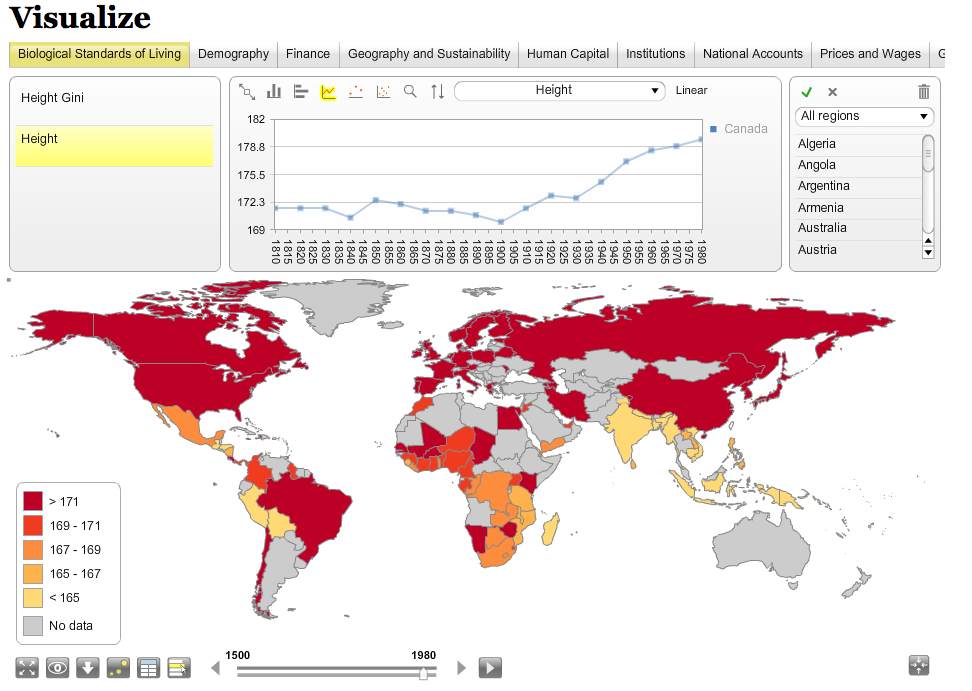
\includegraphics{clio_nlgis01-figure/clio_statplanet_visualize.png}

\end{frame}

\begin{frame}{CLIO-INFRA en Statplanet}

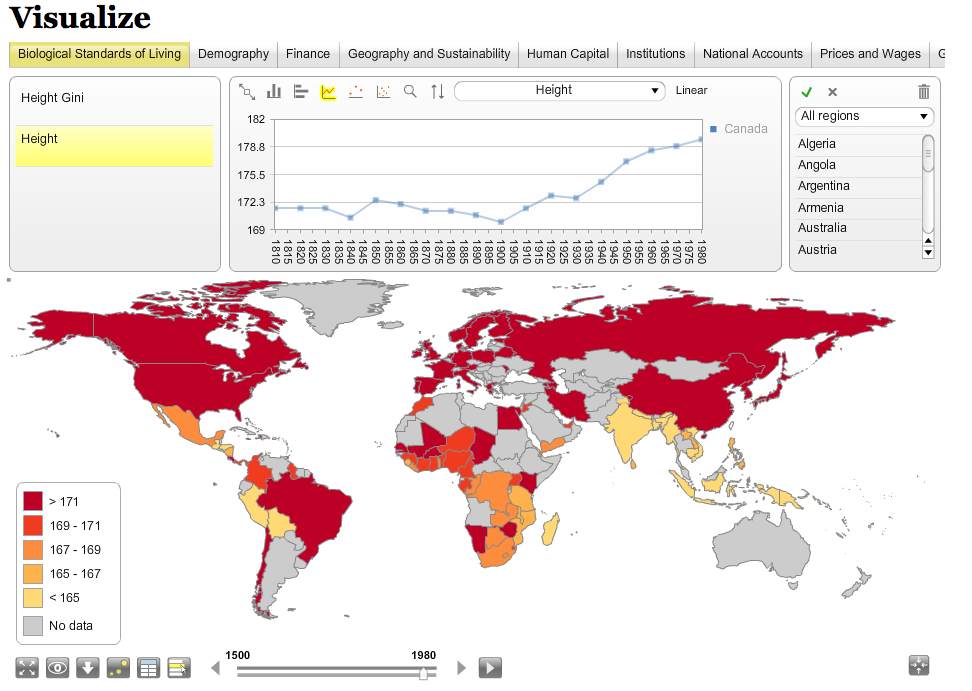
\includegraphics{clio_nlgis01-figure/clio_statplanet_visualize.png}

Veranderingen over de tijd, maar geen historische grenzen

\end{frame}

\begin{frame}{Waarom historisch accurate grenzen?}

\begin{itemize}
\itemsep1pt\parskip0pt\parsep0pt
\item
  inzicht in context (bv. Algerije als Frans grondgrebied)
\item
  beschrijvende analyses (bv. bevolkingsdichtheid)
\item
  verklarende analyses: cluster correctie
\item
  spatiële regressie
\item
  multi-level regressie
\end{itemize}

\end{frame}

\begin{frame}{Historische GIS in Nederland}

\begin{block}{HISGIS.NL}

\begin{itemize}
\itemsep1pt\parskip0pt\parsep0pt
\item
  zeer gedetailleerd (perceel-niveau)
\item
  voor enkele jaren
\end{itemize}

\end{block}

\begin{block}{NLGIS.NL}

\begin{itemize}
\itemsep1pt\parskip0pt\parsep0pt
\item
  gedetailleerd (gemeente-niveau)
\item
  jaarlijkse kaarten voor (1812-1997)
\end{itemize}

\end{block}

\end{frame}

\begin{frame}{NLGIS: een verkenning}

Mogelijkheden van \href{http://nlgis.nl}{NLGIS}

\begin{block}{Voor het brede publiek}

\begin{itemize}
\itemsep1pt\parskip0pt\parsep0pt
\item
  Visualiseren data op historisch accurate gemeentegrenzen
\item
  Visualiseren eigen datasets
\end{itemize}

\end{block}

\begin{block}{Voor data-scientists}

\begin{itemize}
\itemsep1pt\parskip0pt\parsep0pt
\item
  Toegang tot HDNG data via API
\item
  Toegang tot kaarten via API
\end{itemize}

\end{block}

\begin{block}{Voor onderzoekers}

\begin{itemize}
\itemsep1pt\parskip0pt\parsep0pt
\item
  R-package
\item
  makkelijke toegang tot API
\item
  makkelijk interactief kaarten maken
\item
  integratie met geavanceerde analyses in R
\end{itemize}

\end{block}

\end{frame}

\begin{frame}{Stakingen in kaarten: een uitbreiding}

\begin{itemize}
\itemsep1pt\parskip0pt\parsep0pt
\item
  Data: Stakingen vanaf de 14e eeuw
\item
  Kaarten: 4 jaren op wereldniveau
\end{itemize}

\end{frame}

\begin{frame}{Stakingen in kaarten: een uitbreiding}

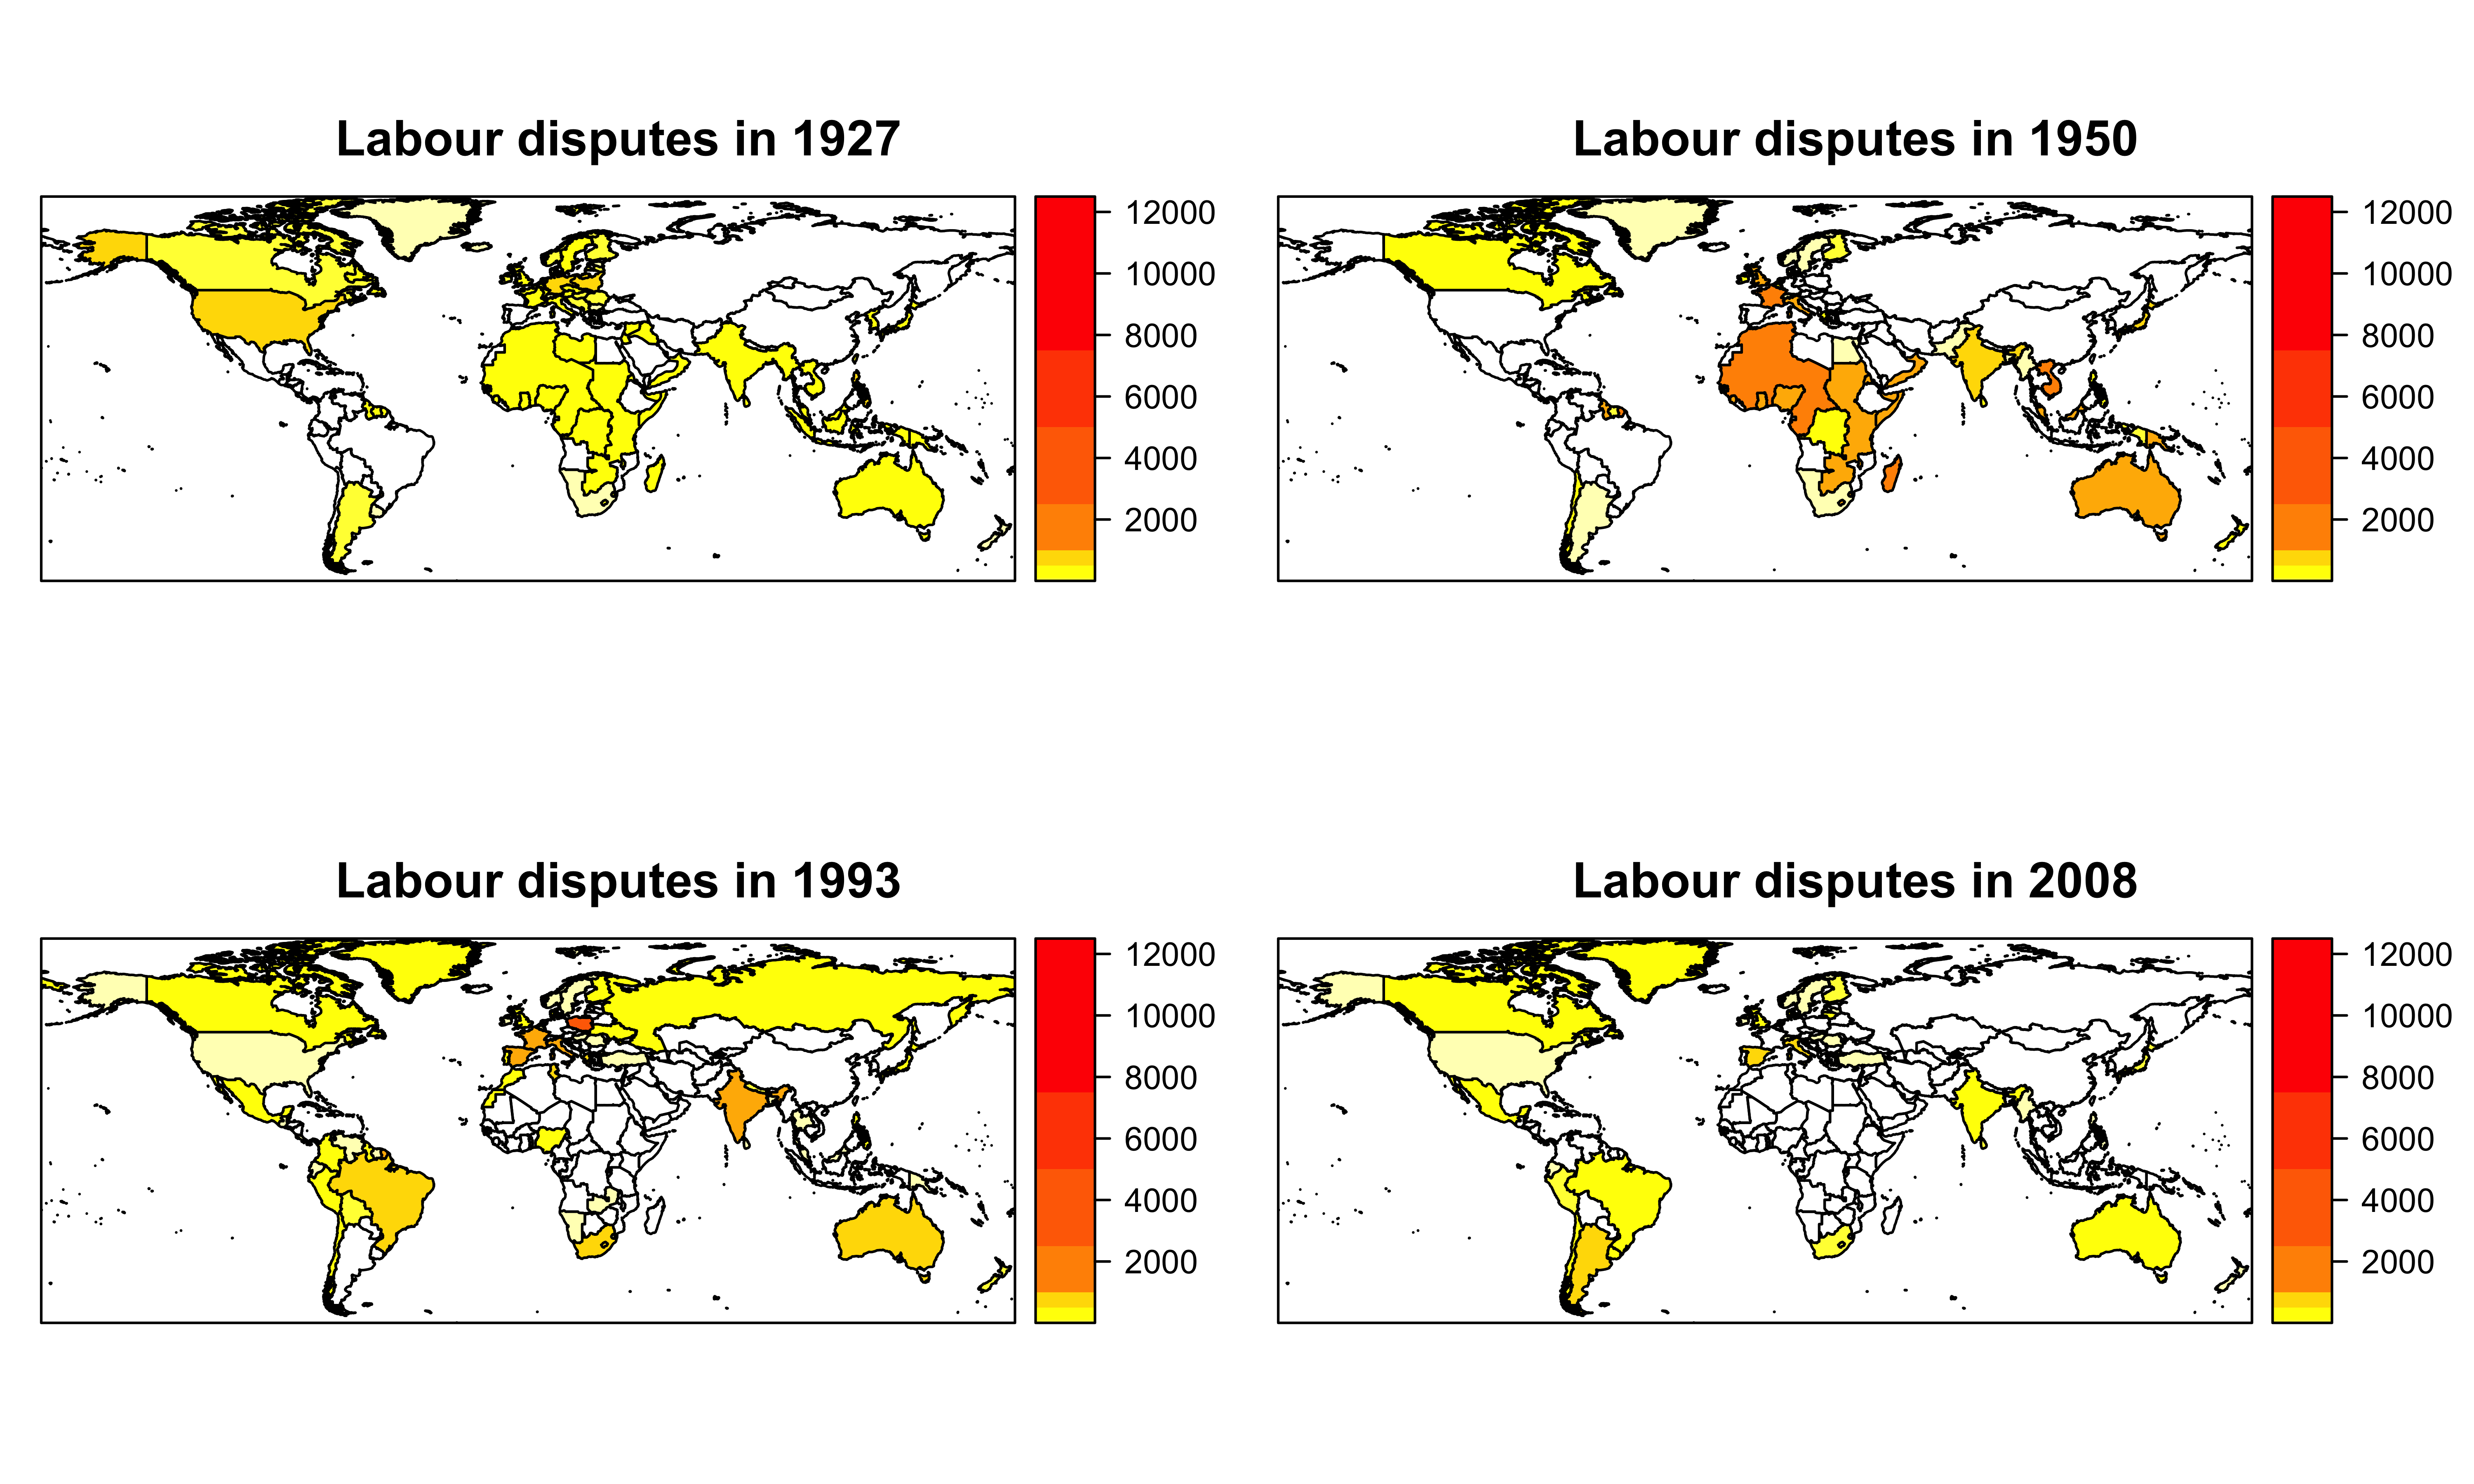
\includegraphics{clio_nlgis01-figure/disputes_changing_boundaries01.png}

\end{frame}

\begin{frame}{Clariah: historische gis infra-structuur}

\begin{itemize}
\itemsep1pt\parskip0pt\parsep0pt
\item
  unieke identificatie van plaats en tijd
\item
  databases geordend op basis van deze identificatie
\item
  visualisatie op historisch accurate kaarten
\item
  implementatie van eenvoudige analyses
\end{itemize}

\end{frame}

\begin{frame}{Contact}

\begin{block}{Richard L. Zijdeman}

\href{mailto:richard.zijdeman@iisg.nl}{richard.zijdeman@iisg.nl}

\end{block}

\end{frame}

\end{document}
